\chapter{Chapter 8: First-Order Logic \& Knowledge Representation}

This chapter compiles high-scoring study notes and complete exam answers for \textbf{Unit VIII: First-Order Logic \& Knowledge Representation} of the OE-EC804A syllabus, adhering strictly to the \textbf{MAKAUT Answer Writing Guidelines}.


\section{Section 1: Declarative vs. Procedural Knowledge and Production Systems (Q8.1)}

\subsection{1. Comparison of Knowledge Types}

\begin{table}[H]
\centering
\begin{tabular}{|p{\dimexpr 0.2\textwidth - 2\tabcolsep - 1.5\arrayrulewidth\relax}|p{\dimexpr 0.4\textwidth - 2\tabcolsep - 1.5\arrayrulewidth\relax}|p{\dimexpr 0.4\textwidth - 2\tabcolsep - 1.5\arrayrulewidth\relax}|}
\hline
Feature & Declarative Knowledge & Procedural Knowledge \\
\hline
\textbf{Definition} & Knowledge that represents static facts, assertions, and concepts about the world. & Knowledge that represents the steps, rules, and procedures to perform a task. \\
\hline
\textbf{Nature} & \textbf{"Knowing what"} (Passive, descriptive facts). & \textbf{"Knowing how"} (Active, procedural steps). \\
\hline
\textbf{Representation} & First-Order Logic, semantic networks, database schemas, frames. & Rules, algorithms, subroutines, step-by-step procedures. \\
\hline
\textbf{Modifiability} & Very easy to add, delete, or update facts independently. & Hard to modify; changes in one step can break subsequent steps. \\
\hline
\textbf{Execution} & Needs an external interpreter or inference engine to process. & Executable directly by the processor/system. \\
\hline
\end{tabular}
\end{table}

\subsection{2. Production Systems in Knowledge Representation}
A \textbf{Production System} is a modular cognitive model of problem-solving consisting of three main components:
\begin{enumerate}
  \item \textbf{Production Rules (Rule Base):} A set of IF-THEN rules of the form:
\end{enumerate}
    \[ \text{IF } \langle\text{Condition/Pattern}\rangle \longrightarrow \text{THEN } \langle\text{Action}\rangle \]
\begin{enumerate}
  \item \textbf{Working Memory (Database):} Holds the current facts and assertions representing the system's current state.
  \item \textbf{Recognize-Act Cycle (Inference Engine):}
\end{enumerate}
    \textit{   }Match:* Compares working memory facts against the IF conditions of production rules.
    \textit{   }Conflict Resolution:* If multiple rules match, a conflict resolution strategy (e.g., recency, specificity, rule priority) selects one rule.
    \textit{   }Act:* Executes the action part of the selected rule, updating the working memory.


\section{Section 2: Horn Clauses and Skolemisation (Q8.2)}

\subsection{1. Horn Clause}
A \textbf{Horn Clause} is a disjunction of literals (clause) containing \textbf{at most one positive (unnegated) literal}. It is the foundation of logic programming (like PROLOG).

There are three types of Horn clauses:
\begin{enumerate}
  \item \textbf{Definite Clause:} Exactly one positive literal (e.g., $\neg p \lor \neg q \lor r$, which is equivalent to $(p \land q) \rightarrow r$).
  \item \textbf{Fact:} A single positive literal with no negative literals (e.g., $p$).
  \item \textbf{Goal Clause:} No positive literals (e.g., $\neg p \lor \neg q$, equivalent to $\neg(p \land q)$).
\end{enumerate}

\subsubsection{Proof: $p \rightarrow q$ is a Horn Clause}
By logical equivalence, the implication $p \rightarrow q$ can be written as:
\[ \neg p \lor q \]
This is a disjunction of literals containing exactly one positive literal ($q$) and one negative literal ($\neg p$). By definition, since it contains at most one positive literal, $p \rightarrow q$ is a \textbf{Horn Clause} (specifically, a definite clause). $\blacksquare$


\subsection{2. Skolemisation}
\textbf{Skolemisation} is the process of eliminating existential quantifiers ($\exists$) in a First-Order Logic formula, replacing them with concrete terms (constants or functions) without changing the satisfiability of the formula.

\subsubsection{Rules for Skolemisation:}
\begin{enumerate}
  \item \textbf{If the existential quantifier is NOT within the scope of any universal quantifier ($\forall$):} Replace the variable with a new, unique constant (a \textbf{Skolem Constant}).
\end{enumerate}
    \textit{   }Example:* $\exists x P(x) \Longrightarrow P(A)$ (where $A$ is a new constant).
\begin{enumerate}
  \item \textbf{If the existential quantifier lies within the scope of one or more universal quantifiers ($\forall$):} Replace the existential variable with a new function (a \textbf{Skolem Function}) whose arguments are the universally quantified variables.
\end{enumerate}
    \textit{   }Example:* $\forall x \exists y Loves(x, y) \Longrightarrow \forall x Loves(x, F(x))$ (where $F(x)$ is a new function mapping each $x$ to its corresponding $y$).


\section{Section 3: PROLOG Programming (Q8.3)}

\subsection{1. Recursive Factorial Program}
\begin{lstlisting}
% Base Case: Factorial of 0 is 1.
factorial(0, 1).

% Recursive Case: Factorial of N (N > 0) is F.
factorial(N, F) :-
    N > 0,
    N1 is N - 1,
    factorial(N1, F1),
    F is N * F1.
\end{lstlisting}

\subsection{2. Recursive Greatest Common Divisor (GCD) Program}
\begin{lstlisting}
% Base Case: GCD of X and 0 is X.
gcd(X, 0, X) :- !.

% Recursive Case: GCD(X, Y) using Euclidean algorithm (modulo operator).
gcd(X, Y, G) :-
    Y > 0,
    R is X mod Y,
    gcd(Y, R, G).
\end{lstlisting}


\section{Section 4: Clausal Form (CNF) and Resolution Refutation Proofs (Q8.4)}

\subsection{1. Step-by-Step Procedure to Convert to CNF}
\begin{enumerate}
  \item \textbf{Eliminate Implications \& Biconditionals:} Replace $A \Rightarrow B$ with $\neg A \lor B$.
  \item \textbf{Move Negations Inward:} Apply De Morgan's laws and double-negation rules (e.g., $\neg(A \land B) \equiv \neg A \lor \neg B$, $\neg \forall x P(x) \equiv \exists x \neg P(x)$).
  \item \textbf{Standardize Variables:} Rename variables so that each quantifier binds a unique variable name.
  \item \textbf{Skolemise:} Eliminate existential quantifiers ($\exists$) using Skolem constants/functions.
  \item \textbf{Drop Universal Quantifiers ($\forall$):} Since all remaining variables are universally quantified, we can drop the quantifiers.
  \item \textbf{Distribute $\lor$ over $\land$:} Structure into Conjunctive Normal Form (CNF) (e.g., $(A \lor B) \land (C \lor D)$).
  \item \textbf{Isolate Clauses:} Write each conjunct as a separate clause.
\end{enumerate}


\subsection{2. CNF Conversion Example}
Convert the following to CNF:
\[ (\forall x)(P(x) \Rightarrow ((\forall y)(P(y) \Rightarrow P(f(x, y))) \land \neg (\forall y)(Q(x, y) \Rightarrow P(y)))) \]

\begin{itemize}
  \item   \textbf{Step 1: Eliminate implications}
\end{itemize}
    \[ (\forall x)(\neg P(x) \lor ((\forall y)(\neg P(y) \lor P(f(x, y))) \land \neg (\forall y)(\neg Q(x, y) \lor P(y)))) \]
\begin{itemize}
  \item   \textbf{Step 2: Move negations inward}
  \item   Focus on $\neg (\forall y)(\neg Q(x, y) \lor P(y))$:
\end{itemize}
        \[ \neg (\forall y)(\dots) \Longrightarrow \exists y \neg(\neg Q(x, y) \lor P(y)) \Longrightarrow \exists y (Q(x, y) \land \neg P(y)) \]
\begin{itemize}
  \item   Reassemble:
\end{itemize}
        \[ (\forall x)(\neg P(x) \lor ((\forall y)(\neg P(y) \lor P(f(x, y))) \land \exists y (Q(x, y) \land \neg P(y)))) \]
\begin{itemize}
  \item   \textbf{Step 3: Standardize variables}
\end{itemize}
    Rename the second $y$ to $z$ to prevent overlap:
    \[ (\forall x)(\neg P(x) \lor ((\forall y)(\neg P(y) \lor P(f(x, y))) \land \exists z (Q(x, z) \land \neg P(z)))) \]
\begin{itemize}
  \item   \textbf{Step 4: Skolemise}
\end{itemize}
    The existential variable $z$ is within the scope of universal quantifier $x$. Replace $z$ with Skolem function $h(x)$:
    \[ (\forall x)(\neg P(x) \lor ((\forall y)(\neg P(y) \lor P(f(x, y))) \land (Q(x, h(x)) \land \neg P(h(x))))) \]
\begin{itemize}
  \item   \textbf{Step 5: Drop universal quantifiers}
\end{itemize}
    \[ \neg P(x) \lor ((\neg P(y) \lor P(f(x, y))) \land Q(x, h(x)) \land \neg P(h(x))) \]
\begin{itemize}
  \item   \textbf{Step 6: Distribute $\lor$ over $\land$}
\end{itemize}
    Apply distributive law: $A \lor (B \land C \land D) \equiv (A \lor B) \land (A \lor C) \land (A \lor D)$.
\begin{itemize}
  \item   \textbf{Clause 1:} $\neg P(x) \lor \neg P(y) \lor P(f(x, y))$
  \item   \textbf{Clause 2:} $\neg P(x) \lor Q(x, h(x))$
  \item   \textbf{Clause 3:} $\neg P(x) \lor \neg P(h(x))$
\end{itemize}


\subsection{3. Resolution Refutation Proof Case Study}
\textit{   }Statements:* "Everyone who enters in a theatre has bought a ticket. Person who does not have money can't buy a ticket. Vinod enters a theatre."
\textit{   }Goal:* Prove that "Vinod has money" ($HasMoney(Vinod)$).

\subsubsection{FOPL Representation:}
\begin{enumerate}
  \item "Everyone who enters in a theatre has bought a ticket":
\end{enumerate}
    \[ \forall x (Enters(x) \rightarrow BoughtTicket(x)) \Longrightarrow \neg Enters(x) \lor BoughtTicket(x) \]
\begin{enumerate}
  \item "Person who does not have money can't buy a ticket":
\end{enumerate}
    \[ \forall y (\neg HasMoney(y) \rightarrow \neg BoughtTicket(y)) \Longrightarrow \text{Implication: } BoughtTicket(y) \rightarrow HasMoney(y) \Longrightarrow \neg BoughtTicket(y) \lor HasMoney(y) \]
\begin{enumerate}
  \item "Vinod enters a theatre":
\end{enumerate}
    \[ Enters(Vinod) \]
\begin{enumerate}
  \item \textbf{Negated Goal:}
\end{enumerate}
    \[ \neg HasMoney(Vinod) \]

\subsubsection{Resolution Proof:}
\textit{   }Step 1:* Resolve Clause 1 ($\neg Enters(x) \lor BoughtTicket(x)$) and Clause 3 ($Enters(Vinod)$) using substitution $\{x/Vinod\}$:
\begin{itemize}
  \item   \textbf{Inferred Clause 5:} $BoughtTicket(Vinod)$
\end{itemize}
\textit{   }Step 2:* Resolve Clause 2 ($\neg BoughtTicket(y) \lor HasMoney(y)$) and Clause 5 ($BoughtTicket(Vinod)$) using substitution $\{y/Vinod\}$:
\begin{itemize}
  \item   \textbf{Inferred Clause 6:} $HasMoney(Vinod)$
\end{itemize}
\textit{   }Step 3:* Resolve Clause 6 ($HasMoney(Vinod)$) and Negated Goal ($\neg HasMoney(Vinod)$):
\begin{itemize}
  \item   \textbf{Inferred Clause 7:} $\Box$ (Empty clause / Contradiction).
  \item   \textbf{Conclusion:} Since the empty clause is derived, the negated goal is false. Thus, \textbf{Vinod has money}. $\blacksquare$
\end{itemize}


\section{Section 5: Predicate Logic Case Study -- Marcus Hated Caesar (Q8.5)}

\subsection{1. FOPL Representation}
\begin{enumerate}
  \item \textit{Marcus was a man:} $Man(Marcus)$
  \item \textit{Marcus was Pompeian:} $Pompeian(Marcus)$
  \item \textit{All Pompeians were Romans:} $\forall x (Pompeian(x) \rightarrow Roman(x)) \Longrightarrow \neg Pompeian(x) \lor Roman(x)$
  \item \textit{Caesar was a ruler:} $Ruler(Caesar)$
  \item \textit{All Romans were either loyal to Caesar or hated him:}
\end{enumerate}
    \[ \forall x (Roman(x) \rightarrow LoyalTo(x, Caesar) \lor Hate(x, Caesar)) \Longrightarrow \neg Roman(x) \lor LoyalTo(x, Caesar) \lor Hate(x, Caesar) \]
\begin{enumerate}
  \item \textit{Everyone is loyal to someone:} $\forall x \exists y LoyalTo(x, y) \Longrightarrow \forall x LoyalTo(x, f(x))$ (where $f(x)$ is a Skolem function).
  \item \textit{People only try to assassinate rulers they are not loyal to:}
\end{enumerate}
    \[ \forall x \forall y (Man(x) \land Ruler(y) \land TryAssassinate(x, y) \rightarrow \neg LoyalTo(x, y)) \]
    \[ \Longrightarrow \neg Man(x) \lor \neg Ruler(y) \lor \neg TryAssassinate(x, y) \lor \neg LoyalTo(x, y) \]
\begin{enumerate}
  \item \textit{Marcus tried to assassinate Caesar:} $TryAssassinate(Marcus, Caesar)$
\end{enumerate}


\subsection{2. Resolution Refutation Proof}
\begin{itemize}
  \item   \textbf{Negated Goal:} $\neg Hate(Marcus, Caesar)$
\end{itemize}

\begin{figure}[H]
\centering
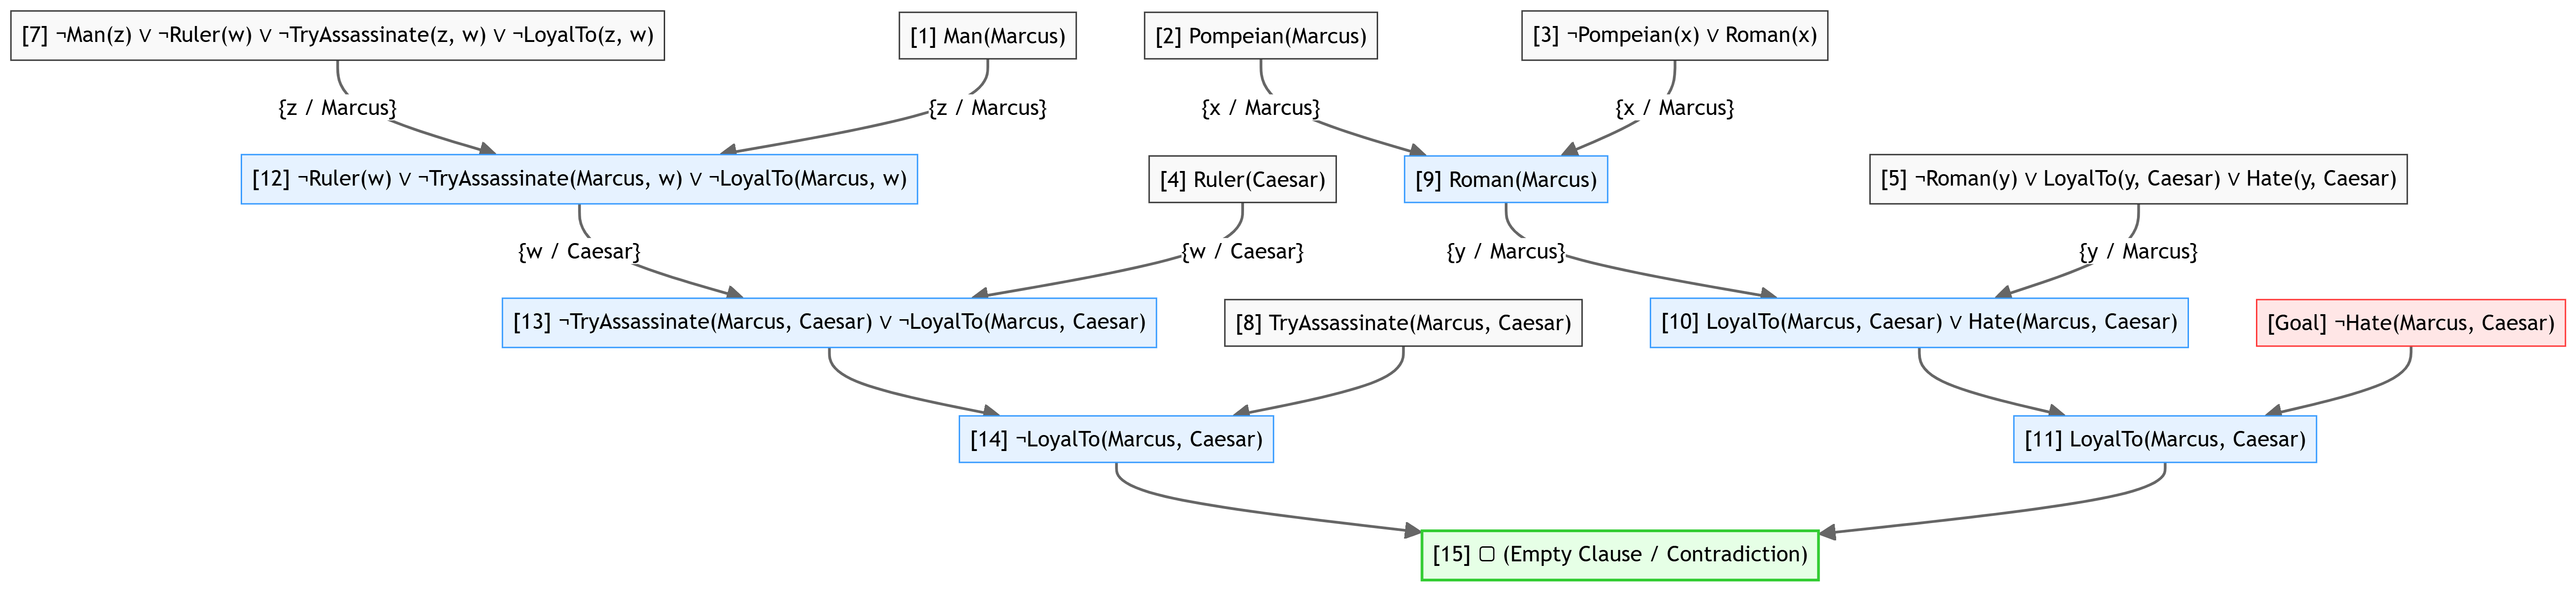
\includegraphics[width=0.75\textwidth,height=0.32\textheight,keepaspectratio]{../Images/chapter_08/resolution_steps.png}
\caption{Resolution Refutation Proof Tree}
\end{figure}

\textbf{Conclusion:} The contradiction proves that the negated goal is false. Therefore, \textbf{Marcus hated Caesar}. $\blacksquare$


\section{Section 6: Knowledge Representation Techniques (Q8.6)}

\subsection{1. Semantic Networks}
\begin{itemize}
  \item   \textbf{Definition:} A graphical representation of knowledge consisting of nodes (objects/concepts) and directed, labeled edges (relations).
\end{itemize}
\textit{   }Sourav is 6 feet tall and is taller than Sachin:*

\begin{figure}[H]
\centering
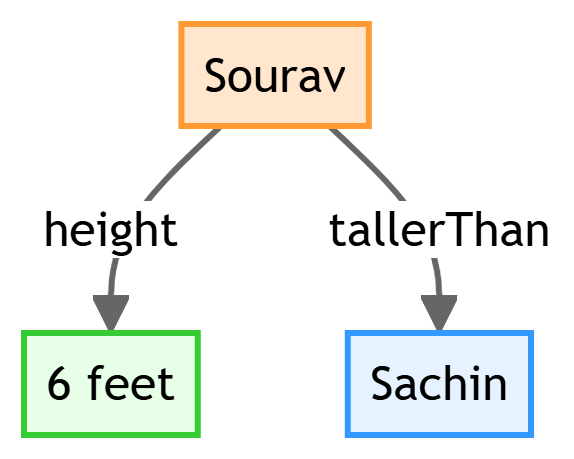
\includegraphics[width=0.75\textwidth,height=0.32\textheight,keepaspectratio]{../Images/chapter_08/semantic_network.png}
\caption{Semantic Network}
\end{figure}


\subsection{2. Frames}
\begin{itemize}
  \item   \textbf{Definition:} A collection of attributes (called \textbf{slots}) and associated values (called \textbf{fillers}) that describe an entity. Support class-inheritance.
  \item   \textbf{Example Frame:}
\end{itemize}
\begin{lstlisting}
Frame: Patient
    isa: Person
    Age: default_value (30)
    Doctor: default_value (Dr. Smith)
    
  Frame: John
    isa: Patient
    Age: 45                 (Inherits Doctor as Dr. Smith; overrides Age to 45)
\end{lstlisting}


\subsection{3. Fuzzy Logic}
\begin{itemize}
  \item   \textbf{Definition:} A form of many-valued logic where truth values are real numbers between $0$ (completely false) and $1$ (completely true), representing degrees of membership in a set.
  \item   \textbf{Fuzzy Set Operations:}
  \item   \textbf{Union ($\cup$):} $\mu_{A \cup B}(x) = \max(\mu_A(x), \mu_B(x))$
  \item   \textbf{Intersection ($\cap$):} $\mu_{A \cap B}(x) = \min(\mu_A(x), \mu_B(x))$
  \item   \textbf{Complement ($\bar{A}$):} $\mu_{\bar{A}}(x) = 1 - \mu_A(x)$
  \item   \textbf{Crisp vs. Fuzzy Set Difference:} A crisp set has binary membership ($\mu(x) \in \{0, 1\}$; an element is either in the set or not), while a fuzzy set allows continuous degrees of membership ($\mu(x) \in [0, 1]$; e.g., a person can be "partially tall" with membership $0.7$).
\end{itemize}


\subsection{4. Neural Networks and Genetic Algorithms}
\begin{itemize}
  \item   \textbf{Hebb's Rule:} A learning rule stating that the weight of a connection between two neurons increases if both neurons are active at the same time ("Neurons that fire together, wire together"):
\end{itemize}
    \[ \Delta w_{ij} = \eta \times a_i \times a_j \]
    Where $\eta$ is learning rate, and $a_i, a_j$ are neuron activations.
\begin{itemize}
  \item   \textbf{Genetic Algorithms Operators:}
  \item   \textbf{Crossover:} Combines genetic material from two parent chromosomes to create offspring (e.g., cutting parents at a point and swapping tails).
  \item   \textbf{Mutation:} Randomly alters one or more gene values in a chromosome (e.g., flipping a bit from 0 to 1) with low probability to maintain genetic diversity.
\end{itemize}
